The Time-dependent Latent Space GPLVM model allows the GPLVM extra flexibility through the stocks representations in latent space having mobility. The distance between the instances in latent space implies higher correlation if it is smaller, and lower correlation if it is larger. We proceed with the same sanity checks and model evaluations as before. It is necessary to note, that the model did not produce symmetric covariance matrices for kernels of the Matern-class. Therefore, these are not part of the evaluation. Also, due to the size of the matrices needed to express this model, only the small data matrix that was used in the V-GPLVM ($N=10$, $D=250$) could be used. 
\begin{figure}[t]
	\centering
	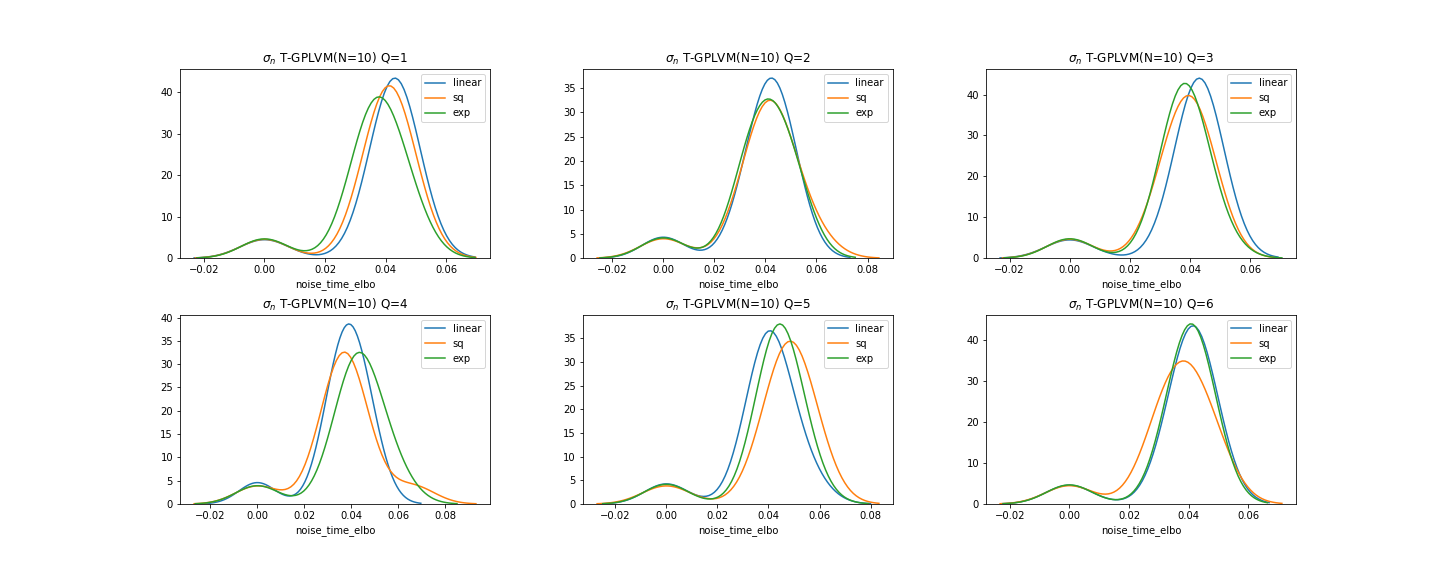
\includegraphics[width=7in]{img/07_3/noise_time_elbo.png}
	\caption[T-GPLVM noise distributions]{T-GPLVM data space ($Y$) observation noise distributions.}
	\label{fig:tgplvm_noise}
\end{figure}
\begin{figure}[b]
	\centering
	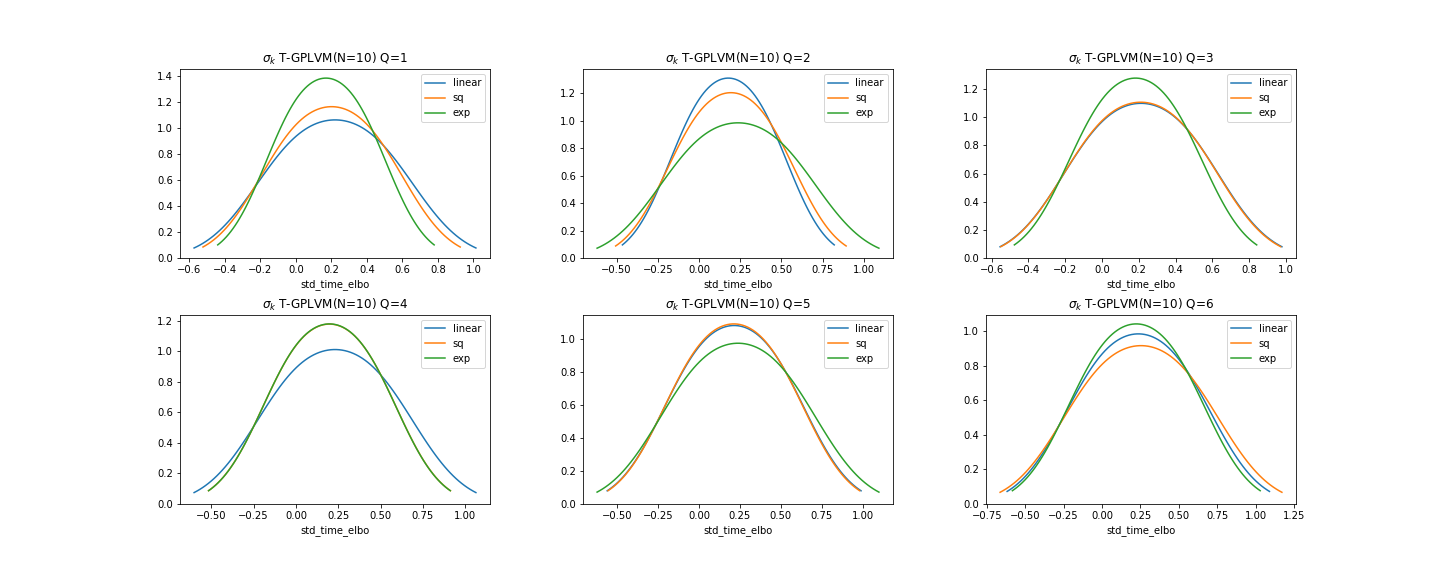
\includegraphics[width=7in]{img/07_3/std_time_elbo.png}
	\caption[T-GPLVM variance distributions]{T-GPLVM data space ($Y$) variance distributions.}
	\label{fig:tgplvm_variance}
\end{figure}
\begin{figure}[t]
	\centering
	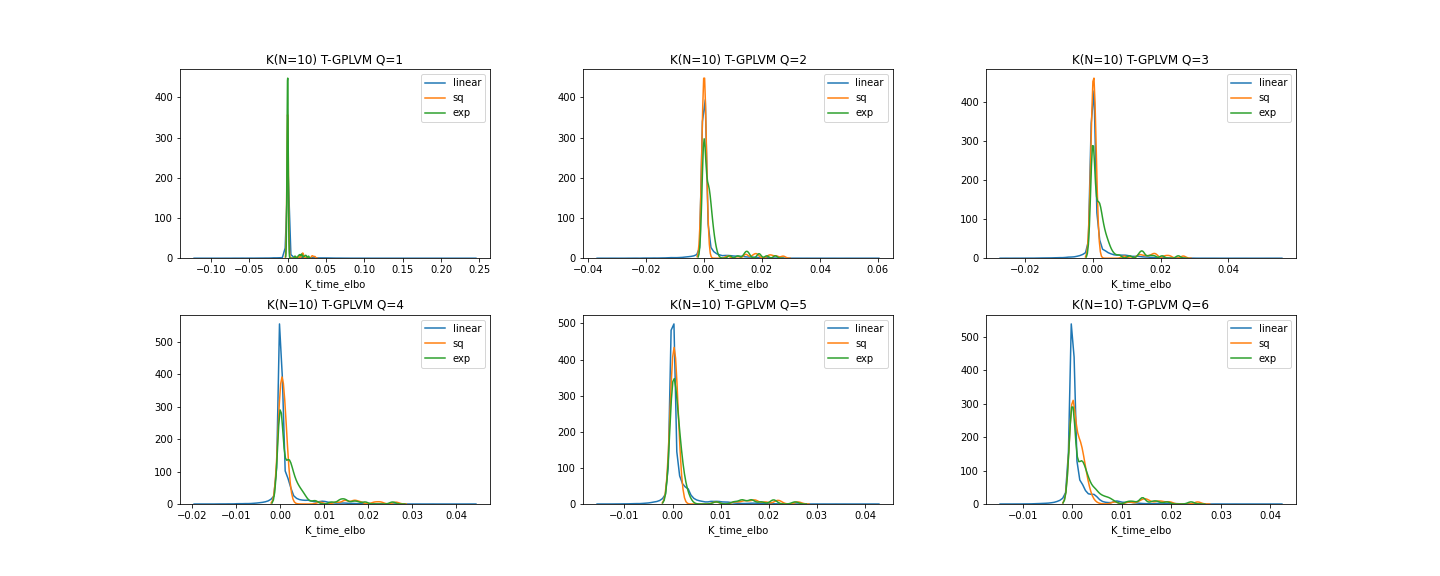
\includegraphics[width=7in]{img/07_3/K_time_elbo.png}
	\caption[T-GPLVM covariance matrix entries distributions]{Covariance matrix entries distributions from the T-GPLVM model run.}
	\label{fig:tgplvm_covariance}
\end{figure}
Figure \ref{fig:tgplvm_noise} shows good agreement with expectations, observation noise is comparably low for all different versions of the model. On the other hand figure \ref{fig:tgplvm_variance}, displaying the variance, shows erroneous behavior, and probably would have been better approximated with some other, most likely asymmetric distribution. At last figure \ref{fig:tgplvm_covariance} shows values close to 0 dominating, implying comparably small covariance between stocks.
\begin{figure}[b]
	\centering
	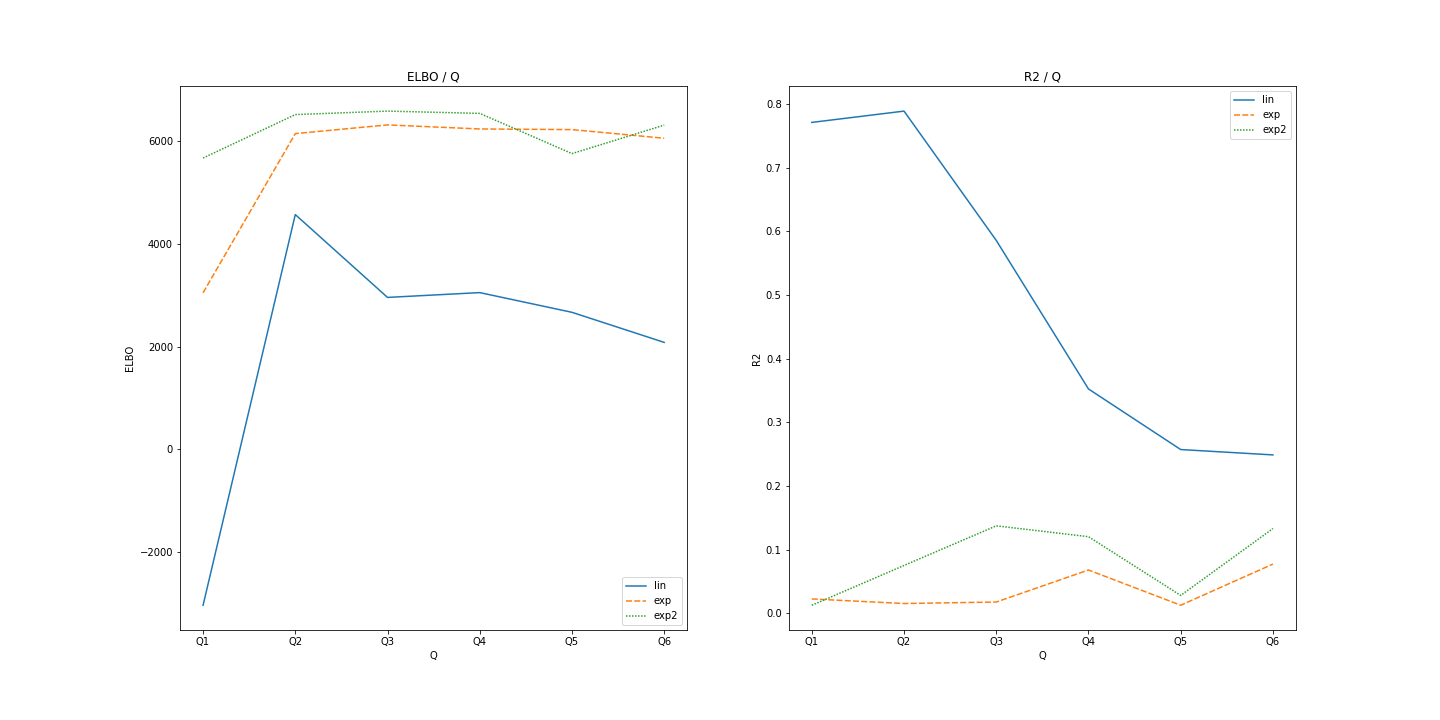
\includegraphics[width=7in]{img/07_3/modelTIME_Qs.png}
	\caption[T-GPLVM ELBO and $R^2$ results]{ELBO and $R^2$ values from the T-GPLVM model run, without the Matern class kernels.}
	\label{fig:tgplvm_ELBO_R2}
\end{figure}
Figure \ref{fig:tgplvm_ELBO_R2} then provides a problem of interpretation. While the ELBO values of the linear kernel are lower, the lower dimensional representation of the reconstruction in form of the $R^2$ values is considerably higher for the linear kernel. Overarching still is the fact, that the ELBO values and $R^2$ values still can not compete with the GPLVM model, just like the V-GPLVM model. 
\begin{figure}[t]
	\centering
	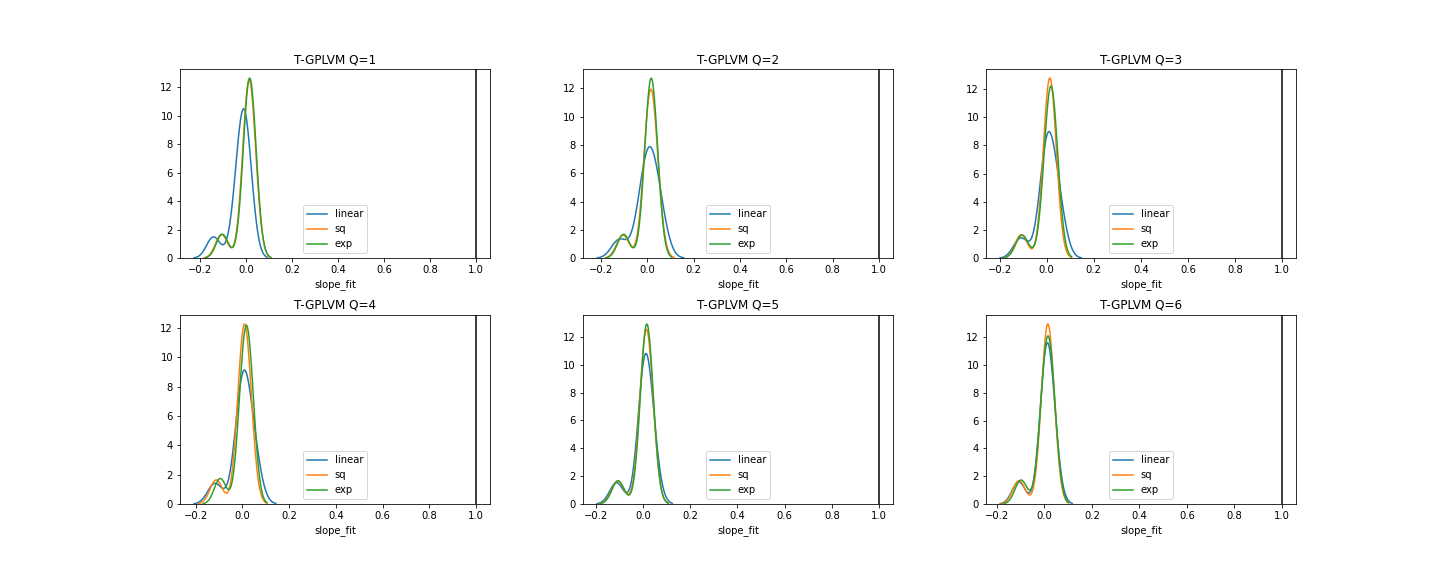
\includegraphics[width=7in]{img/07_3/slope_fit_time_elbo.png}
	\caption[T-GPLVM slope distributions]{Distributions of slopes from the Y-$\hat{Y}$ pairs for the T-GPLVM model.}
	\label{fig:tgplvm_slopes}
\end{figure}
\begin{figure}[b]
	\centering
	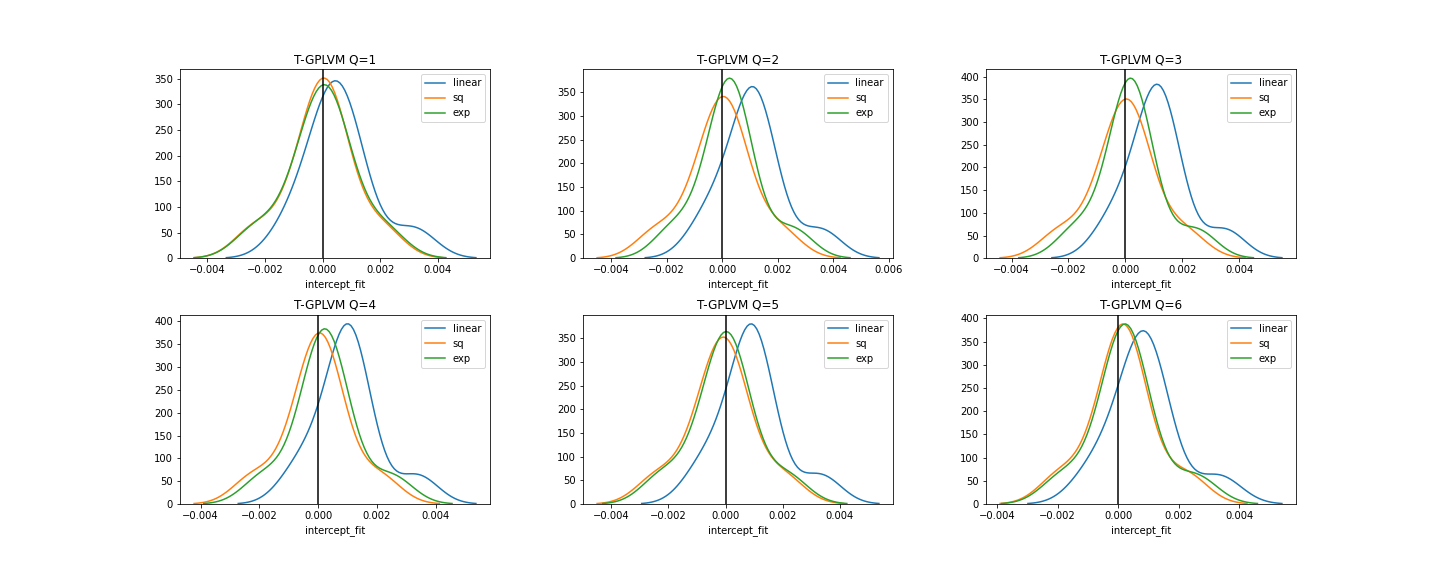
\includegraphics[width=7in]{img/07_3/intercept_fit_time_elbo.png}
	\caption[T-GPLVM intercept distributions]{Distributions of intercepts from the Y-$\hat{Y}$ pairs for the T-GPLVM model.}
	\label{fig:tgplvm_intercepts}
\end{figure}
This conclusion is further exemplified in figures \ref{fig:tgplvm_slopes} and \ref{fig:tgplvm_slopes}, where intercepts can compete with the other models, but slopes of the Huber regression still produce distributions with values so far off from the desired value. Last, but not least, evaluating some examples of the Y-$\hat{Y}$-pair plots makes abundantly clear, that the model still has issues in need to be fixed. All examples show, that distributions match only in lower dimensional representations. The covariance structure of 10 stocks was not enough to be representative of the underlying structure. 
\begin{figure}[t]%fig:gplvm_N120_pairs
	\centering
	\begin{subfigure}[l]{0.3\textwidth}
		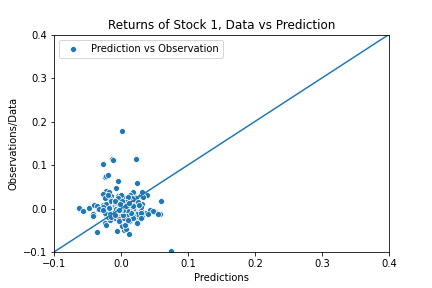
\includegraphics[width=\textwidth]{img/07_3/Q1_kernel1_stock1_scatter.png}
	\end{subfigure}
	\begin{subfigure}[c]{0.3\textwidth}
		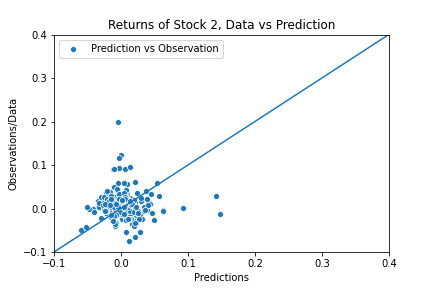
\includegraphics[width=\textwidth]{img/07_3/Q1_kernel1_stock2_scatter.png}
	\end{subfigure}
	\begin{subfigure}[r]{0.3\textwidth}
		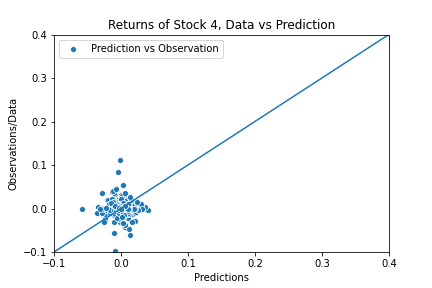
\includegraphics[width=\textwidth]{img/07_3/Q2_kernel1_stock4_scatter.png}
	\end{subfigure}
	\caption[Y-$\hat{Y}$ pair plots for N=10 with the T-GPLVM model]{Plots from the T-GPLVM reconstruction with the $N=10$, $D=250$ dataset.}
	\label{fig:T-Gplvm_pairs}
\end{figure} 